\documentclass[9pt,conference]{IEEEtran}
\usepackage[english]{babel}
\usepackage[utf8]{inputenc}
\usepackage{amssymb}
\usepackage{amsmath}

\usepackage[maxnames=5, sorting=none]{biblatex}

% Text
\newcommand{\rv}{r.v.}
\newcommand{\rvs}{r.v.'s}

\newcommand{\ie}{\emph{i.e.}}
\newcommand{\eg}{\emph{e.g.}}
\newcommand{\etc}{\emph{etc.}}
\newcommand{\apriori}{\emph{a priori}}

% References
\newcommand{\eref}[1]{Eq.~(\ref{equ:#1})}
\newcommand{\sref}[1]{Sec.~\ref{sec:#1}}

\newcommand{\elabel}[1]{\label{equ:#1}}
\newcommand{\slabel}[1]{\label{sec:#1}}

% Sets
\newcommand{\real}{\mathbb{R}}

% Linear algebra
\newcommand{\m}[1]{\mathbf{#1}}
\renewcommand{\v}[1]{\mathbf{#1}}

\newcommand{\vZero}{\mathbf{0}}

% Theory of probability
\newcommand{\outcomes}{\Omega}
\renewcommand{\o}{\omega}
\newcommand{\salgebra}{\mathcal{F}}
\newcommand{\pmeasure}{\mathcal{P}}

\newcommand{\U}{U}
\newcommand{\vU}{\v{U}}

\newcommand{\normal}[2]{\mathcal{N}\left(#1, #2\right)}

% System
\newcommand{\model}[1]{\mathcal{M}\left(#1\right | \vU(\o))}

% Temperature
\newcommand{\specification}{\mathcal{S}}

\newcommand{\T}{\Theta}
\newcommand{\vT}{\boldsymbol\Theta}
\newcommand{\mT}{\boldsymbol\Theta}
\newcommand{\amb}{\text{amb}}
\newcommand{\meas}{\text{meas}}

% Power
\renewcommand{\P}{P}
\newcommand{\vP}{\v{P}}
\newcommand{\mP}{\m{P}}
\newcommand{\dyn}{\text{dyn}}
\newcommand{\leak}{\text{leak}}

% Time
\renewcommand{\t}{t}
\newcommand{\dt}{\Delta \t}
\newcommand{\period}{\tau}

% Profiles
\newcommand{\partition}{\boldsymbol{\Delta}}
\newcommand{\profile}[1]{\left(\partition, #1\right)}

\makeatletter
\def\profileP{\@ifnextchar\bgroup{\profilePWithArgument}{\profilePWithoutArgument}}
\def\profilePWithArgument#1{\profile{\mP(#1)}}
\def\profilePWithoutArgument{\profile{\mP}}

\newcommand{\profilePdyn}{\profile{\mP_\dyn}}

\def\profileT{\@ifnextchar\bgroup{\profileTWithArgument}{\profileTWithoutArgument}}
\def\profileTWithArgument#1{\profile{\mT(#1)}}
\def\profileTWithoutArgument{\profile{\mT}}
\makeatother

\newcommand{\profileTmeas}{\profile{\mT_\meas}}

\newcommand{\profilePT}{\profile{\mP, \mT}}
\newcommand{\profilePdynT}{\profile{\mP_\dyn, \mT}}

\newcommand{\data}{\mathcal{D}}

% Uncertainties
\newcommand{\noise}{\N}
\newcommand{\mnoise}{\v{N}}
\newcommand{\vnoise}{\m{N}}

\newcommand{\mSigma}{\boldsymbol\Sigma}

% Numbers
\newcommand{\ncores}{{N_\text{p}}}
\newcommand{\nsteps}{N_\text{s}}
\newcommand{\ndata}{N_\text{d}}


\bibliography{include/references.bib}

\begin{document}
  \title{Uncertainty Quantification of Process Variation Based on Indirect, Incomplete, and Noisy Measurements\vspace{-1em}}

  \author{
    % \IEEEauthorblockN{Ivan Ukhov}
\IEEEauthorblockA{Link\"{o}ping University\\Sweden\\ivan.ukhov@liu.se}
\and
\IEEEauthorblockN{Mattias Villani}
\IEEEauthorblockA{Link\"{o}ping University\\Sweden\\mattias.villani@liu.se}
\and
\IEEEauthorblockN{Petru Eles}
\IEEEauthorblockA{Link\"{o}ping University\\Sweden\\petru.eles@liu.se}
\and
\IEEEauthorblockN{Zebo Peng}
\IEEEauthorblockA{Link\"{o}ping University\\Sweden\\zebo.peng@liu.se}

  }

  \maketitle

  \begin{abstract}
    In this paper, we propose and develop a novel multiprocessor system design framework for the analysis of process variations across semiconductor wafers. Instead of taking direct measurements of the quantity of interest being characterized, our technique operates on indirect observations, namely, on temperature profiles, which are cheap to collect as no deployment of expensive test structures is required.
The experimental results provide a comprehensive study of our approach for a wide range of configurations having high practical importance.

  \end{abstract}

  \section{Introduction and Prior Work} \slabel{introduction}
  Process variation is one of the major concerns of multiprocessor system architects. The crucial implication of process variation is that it renders the key parameters of a technological process, \eg, the effective channel length, gate oxide thickness, threshold voltage, \etc, as random variables (\rvs). Hence, a deterministic workload of the multiprocessor platform at hand results in stochastic power and, consequently, temperature profiles as they essentially depend on those key parameters; in other words, power and temperature of two ``identical'' dies, performing the same operation, vary. This phenomenon leads to performance degradation and, in the worst case, to burnt chips. Therefore, the concept of uncertainty quantification (UQ) has become central for the multiprocessor system design workflows that are concerned with efficiency and robustness of their products. In this paper, we consider an inverse UQ problem targeted at inferring the parameters that are deteriorated by process variation based on a data set of measurements, which we analyze using Bayesian inference \cite{gelman2004}.

Bayesian inference is utilized in \cite{zhang2010} to identify an optimal set of spatial locations on the wafer, in which the quantity of interest (QoI), such as the effective channel length, should be measured in order to characterize it with the maximal accuracy. In \cite{paek2012}, the authors address the inference of the power dissipation based on transient temperature profiles using Markov random fields. Another temperature-based characterization of power is developed in \cite{mesa-martinez2007} wherein a genetic algorithm is employed for reconstruction of the power model. It should be noted that the approach in \cite{zhang2010} requires measurement structures to be deployed onto each die on the wafer as it operates on direct observations of the QoI. This can be expensive and, thus, impractical to undertake. The techniques in \cite{paek2012} and \cite{mesa-martinez2007} solely focus on power and do attempt to infer other parameters.

The contribution of our work is in the following. We propose a novel approach to UQ of process variation based on indirect, incomplete, and noisy measurements. Indirectness is the key ingredient of our technique: instead of measuring the QoI directly, we propose to measure temperature.

The reminder of this paper is organized as follows. In \sref{problem-formulation}, we formulate the objective of our study. Preliminary materials are given in \sref{preliminaries}. The proposed UQ framework is presented in \sref{proposed-framework}. Experimental results are reported in \sref{experimental-results}. \sref{conclusion} concludes the paper.


  \section{Motivational Example} \slabel{motivation}
  \begin{figure}[b!]
  \vspace{-2em}
  \centering
  \subfloat[True QoI.]{
    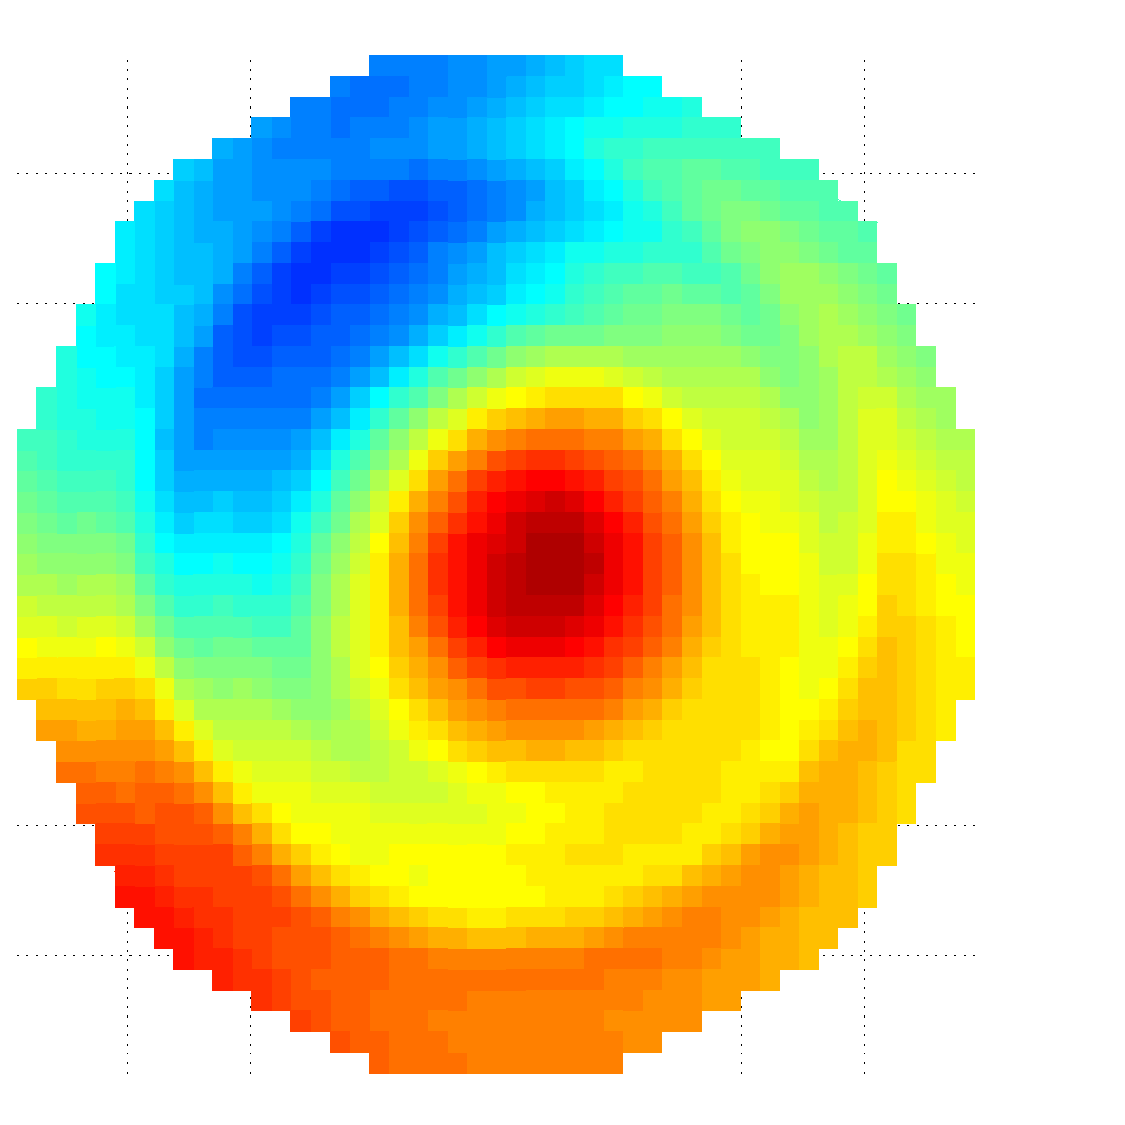
\includegraphics[width=0.4\linewidth]{include/assets/wafer-qoi-true.pdf}
    \flabel{wafer-qoi-true}
  }
  \subfloat[Inferred QoI.]{
    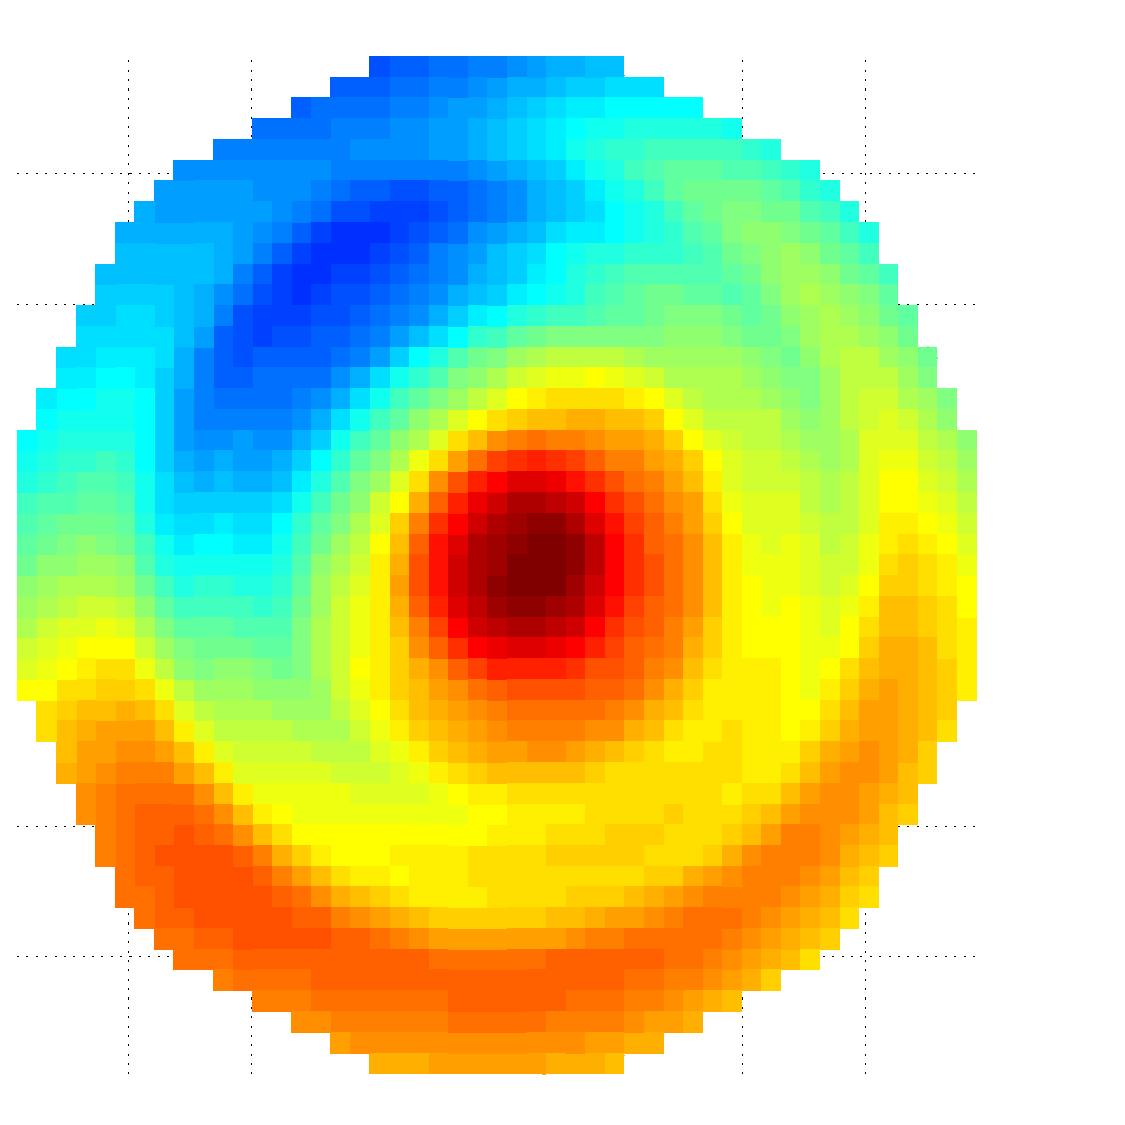
\includegraphics[width=0.4\linewidth]{include/assets/wafer-qoi-inferred.pdf}
    \flabel{wafer-qoi-inferred}
  }
  \caption{The distribution of the QoI across the wafer.}
\end{figure}

Let us consider an example that illustrates an important application of the proposed technique. As previously mentioned, due to process variation, the key parameters that have direct impacts on power and temperature are intrinsically uncertain. Let $\u$ be one of such uncertain quantities; say, the effective channel length.
Assume the technological process imposes a lower bound $\u_*$ on $\u$. This bound separates defective dies ($\u < \u_*$) from those that function properly ($\u_* \leq \u$).
In order to reduce costs, the manufacturer is interested in detecting the faulty dies and taking them out of the production pipeline at early stages. Then, the possible actions that they might take with respect to a single die on the wafer are: (a) keep the die if it closely conforms to the specification; (b) recycle the die, otherwise.
Let the distribution of $\u$ across the wafer be the one depicted on the left side of \fref{wafer-qoi} where the gradient from navy to dark red represents the transition of $\u$ from low to high values.\footnote{The experimental setup is described in detail in \sref{experimental-results}.}
A common approach to find this distribution is to deploy adequate test structures on the dies and measure $\u$ directly; then, an appropriate decision can be taken using the collected information. The problem in this scenario, however, is that the described procedure is technologically complex and, thus, might significantly increase the production costs.

The technique developed in this paper works differently. We apply a fixed workload to a small number of dies on the wafer and measure the corresponding temperature profiles. These profiles can be coarse (low frequency of sampling) and can potentially be corrupted by the measurement noise. Since temperature is cheap to track using, \eg, infrared cameras and no on-die test structures are required, our approach can considerably decrease the costs associated with the characterization of process variation and further decision making.
The result of our framework applied to a data set with less than $7\%$ of the dies on the wafer is shown on the right side of \fref{wafer-qoi}. It can be seen that the two fields closely match each other.

The proposed framework can readily be utilized to estimate probabilities of various events, \eg, $\probabilityMeasure(\u < \u_*)$. This fact is important since, in reality, we do not know the true values and, therefore, can reason about our decisions only in terms of probabilities. We can then reformulate the decision rule defined earlier as follows: (a) keep the die if $\probabilityMeasure(\u_* \leq \u)$ is larger than a certain threshold; (b) recycle the die, otherwise.
An illustration of this rule is given in \fref{wafer-defect} where the threshold is set to two standard deviation below the mean value of $\u$, the crosses mark defective dies (the navy areas in \fref{wafer-qoi}), and the gradient from light gray to red corresponds to the inferred probability of a die to be defective. It can be seen that the inference accurately detects faulty regions.
\begin{figure}[t!]
  \centering
  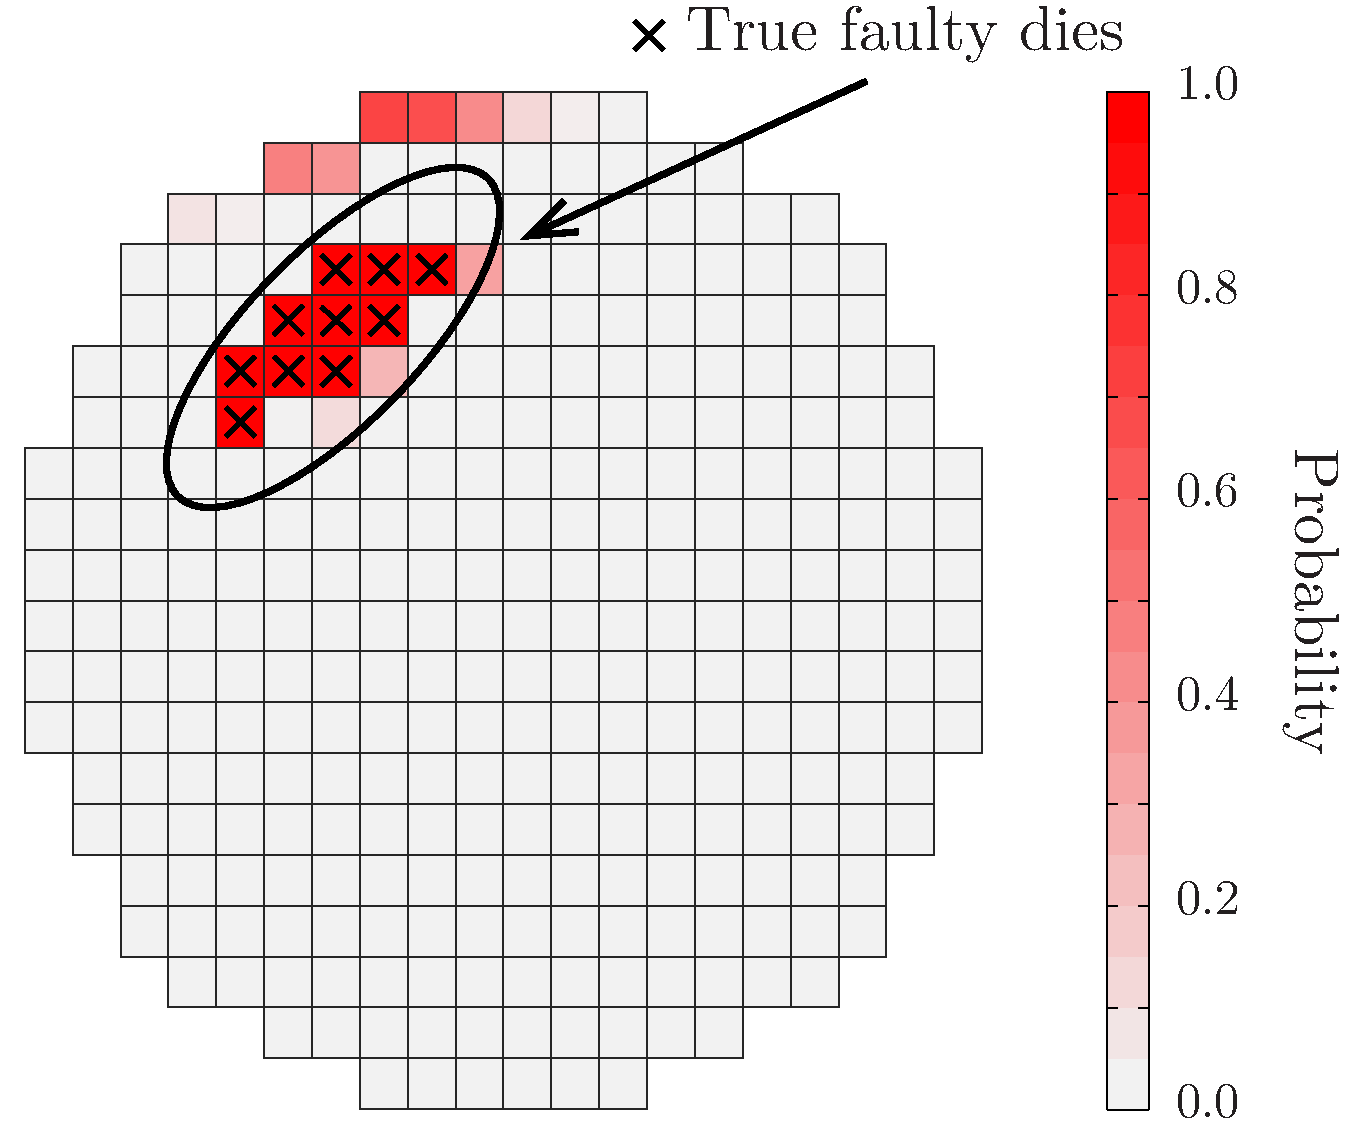
\includegraphics[width=0.6\linewidth]{include/figures/wafer-defect.pdf}
  \caption{Inferred probability of defective dies.}
  \flabel{wafer-defect}
  \vspace{-1.5em}
\end{figure}


In addition, we can introduce a trade-off action: (c) expose the die to a thorough inspection (\eg, via a test structure) if $\probabilityMeasure(\u_* \leq \u)$ is smaller than the threshold of (a) and is larger than some other threshold. In this case, we can reduce costs by examining only those dies for which there is no strong evidence of their satisfactory or unsatisfactory condition.
Furthermore, one can introduce in the inference a so-called utility function, which, for each combination of an outcome of $\u$ and a taken action, assigns the corresponding amount of gain that the decision maker obtains. Then, the inference path, taken in this paper (Bayesian inference), can lead to such an action that maximized the expected utility with respect to the posterior distribution of $\u$. In other words, all possible outcomes of $\u$ weighted by their probabilities will be taken into account in our final decision.


  \section{Problem Formulation} \slabel{problem-formulation}
  Consider a generic electronic system, which is fabricated on a silicon wafer hosting $\ndies$ dies.
The system depends on a process parameter $\u$, which we are interested in studying and shall refer to as the quantity of interest (\qoi).
Due to the presence of process variation, the value of $\u$ deviates from the nominal one, and this deviation can be different at different locations on the wafer.
The \qoi\ is assumed to be impractical for direct measurements.

The goal of this work is to develop a statistical framework targeted at the identification of the on-wafer distribution of $\u$ with the following properties: (a) low measurement costs; (b) high computational speed; (c) robustness to the measurement noise; (d) ability to assess the trustworthiness of the collected data and corresponding predictions; and (e) ability to accommodate prior knowledge on $\u$.

In order to achieve the aforementioned goal, we propose the use of indirect measurements.
Specifically, instead of $\u$, we measure an auxiliary parameter $\q$, which we shall refer to as the quantity of measure (\qom).
The observations of $\q$ are then processed via Bayesian inference in order to derive the distribution of the \qoi, $\u$.
The \qom\ is chosen such that: (a) $\q$ is convenient and cheap to be tracked; (b) $\q$ depends on $\u$, which is signified by $\q = \oBB{\u}$; and (c) there is a way to compute $\q$ for a given $\u$.
The last means that $\oBB$ should be known; however, it does not have to be explicitly given: our framework uses $\oBB$ as a ``black box''.
For example, $\oBB$ can be a piece of code or an output of an adequate simulator.

As the first step, the user of the proposed framework is supposed to harvest a set of observations of $\q$ at several locations on the wafer (recall \sref{motivation}).
Without loss of generality, we shall adhere to the following convention.
One die corresponds to one potential measurement site, and $\nrdies \ll \ndies$ denotes the number of those sites that have been selected for measurements.
Each site comprises $\nprocs$ measurement points, and each point contains $\nsteps$ data instances.
For example, in \sref{motivation}, each observation was an $\nprocs \times \nsteps$ matrix capturing temperature of $\nprocs$ processing elements for $\nsteps$ moments of time.
Denote by $\QData = \{ \q_i^\meas \}_{i = 1}^\nrdies$ the collected data set where $\q_i^\meas \in \real^{\nprocs \times \nsteps}$ stands for one observation of the \qom.
It is implied that the placement of each selected site is recorded along with $\QData$.

For convenience, we denote by $\specification$ all the information relevant to the production and measurement processes including: (a) the layout of the wafer and (b) the floorplan of a die on the wafer.


  \section{Preliminaries} \slabel{preliminaries} \slabel{bayesian-inference}
  \subsection{Bayesian Inference}
As mentioned in \sref{introduction}, the data analysis performed in this work is based on Bayes' rule \cite{gelman2004}:
\[
  \f{\U | \data} = \frac{\f{\data | \U} \f{\U}}{\f{\data}}
\]
where $\f{\cdot}$ and $\f{\cdot | \cdot}$ denote a probability density function (\pdf) and a conditional \pdf\ \cite{durrett2010}, respectively. $\f{\U}$ is known as the prior distribution of the parameters $\vU$, $\f{\U | \data}$ is the corresponding posterior distribution, $\f{\data | \U}$ is the likelihood function, and $\f{\data}$ is a normalization constant.

\subsection{Polynomial Chaos}
Denote $\lpspace$ the space of square-integrable \rvs\ defined on $\pspace$. Let $X$ be a \rv\ and denote $\f{x}$ the density of $X$. For clarity of presentation, $X$ is assumed to be one-dimensional. $\lpspace$ is a Hilbert space with the inner product defined as
\begin{equation} \elabel{inner-product}
  \iprod{f(X)}{g(X)} = \E{f(X) g(X)} = \int f(x) g(x) \f{x} dx
\end{equation}
where $\E{\cdot}$ denotes the expected value with respect to $\f{x}$. The corresponding norm of the space is then $\norm{\cdot} = \sqrt{\iprod{\cdot, \cdot}}$. Let $f(X)$ be a functional of $X$. If $f(X) \in \lpspace$, $f(X)$ admits the following expansion, which is convergent in the mean-square sense \cite{maitre2010}:
\[
  f(X) = \sum_{i = 0}^\infty \iprod{f(X)}{\pcb_i(X)} \pcb_i(X).
\]
In the above decomposition, $\{ \pcb_i \}_{i = 0}^\infty$ is a basis in $\lpspace$ composed of univariate polynomials orthogonal with respect to $\f{x}$; in other words,
\[
  \iprod{\pcb_i(X), \pcb_j(X)} = \norm{\pcb_i}^2 \delta_{ij}
\]
where $\delta_{ij}$ is the Kronecker delta function. The multidimensional construction of PC expansions is straightforward and is based on tensor products of the one-dimensional counterparts; see, \eg, \cite{maitre2010}. In the $n$-dimensional case, the inner product in \eref{inner-product} is an $n$-dimensional integral, and the basis functionals $\{ \pcb_i \}_{i = 0}^\infty$ are polynomials of $n$ variables.


  \section{Proposed Framework} \slabel{proposed-framework}
  In this section, we present our framework for the temperature-based characterization of process variation.

\subsection{Forward Model} \slabel{forward-model} \slabel{power-model} \slabel{thermal-model}
The total dissipation of power of a system with $\nprocs$ processing elements at time $\t$ is composed of the dynamic and leakage parts:
\begin{equation} \elabel{total-power}
  \vP(\t, \vT(\t), \u) = \vP_\dyn(\t) + \vP_\leak(\vT(\t), \u)
\end{equation}
where $\vP, \vT \in \real^\nprocs$ are vectors of power and temperature, respectively, and $\u$ is an outcome of the uncertain parametrization. The dynamic part, $\vP_\dyn$, is temperature-independent whereas the leakage part, $\vP_\leak$, is a strong function of the operating temperature.
The influence of process variation on the dynamic power is known to be negligibly small \cite{srivastava2010, juan2011, juan2012}; therefore, only leakage is assumed to be dependent on $\u$.
The choice of the leakage model is irrelevant for the present paper and, therefore, will not be discussed any further.


Given a thermal specification $\specification$ (see \sref{problem-formulation}), an equivalent thermal RC circuit with $\nnodes$ thermal nodes is constructed \cite{kreith2000}. The structure of the circuit depends on the intended level of granularity and, therefore, impacts the resulting accuracy. For clarity of presentation, we assume that each processing element is mapped onto one corresponding node, and the thermal package is represented as a set of additional nodes.

The thermal behavior of the circuit is modeled with the following system of differential-algebraic equations:
\begin{subnumcases}{\elabel{thermal-system}}
  \mC \: \frac{d\vX(\t)}{d\t} + \mG \: \vX(\t) = \mM \: \vP(\t, \vT(\t), \u) \elabel{heat-de} \\
  \vT(\t) = \mM^T \vX(\t) + \vT_\amb \elabel{temperature-output}
\end{subnumcases}
where $\mC \in \real^{\nnodes \times \nnodes}$ is a diagonal matrix of the thermal capacitance; $\mG \in \real^{\nnodes \times \nnodes}$ is a symmetric, positive-definite matrix of the thermal conductance; $\vX \in \real^\nnodes$ is the internal state vector; $\vP \in \real^\nprocs$ and $\mM \in \real^{\nnodes \times \nprocs}$ are the input power vector and its mapping matrix to the thermal nodes; $\vT \in \real^\nprocs$ is the temperature vector, and $\vT_\amb \in \real^\nprocs$ is the vector of the ambient temperature. In general, \eref{heat-de} does not have a closed-form solution due to the power term defined in \eref{total-power}; hence, the system is typically being solved numerically. Consequently, given a dynamic power profile $\profilePdyn$ and using \eref{total-power} and \eref{thermal-system}, we can compute the corresponding temperature profile $(\mT, \partition{\mP})$ where $\mT = (\vT(\t_i))$, $\t_i \in \partition{\mP}$.

Let $\mvT_\meas := \vectorize{\{\mT^{(i)}_\meas\}_{i = 1}^\ndata}$ be the vectorization of the temperature measurements $\{ \mT^{(i)}_\meas \}_{i = 1}^\ndata$ in $\Data$ into a single vector with $\ndps = \ndata \nprocs \nsteps$ entries. For convenience, denote the forward model developed so far by
\begin{equation} \elabel{model}
  \mvT = \model{\u},
\end{equation}
which, for an outcome $\u$, transforms the test dynamic power profile $\profilePdyn$ into the temperature vector $\mvT := \vectorize{\{\mT^{(i)}\}_{i = 1}^\ndata}$ evaluated at the same spatial locations $\vr$ as the vector $\mvT_\meas$ defined earlier.


\slabel{analytical-solution}
The thermal model above is computationally expensive as it involves a system of nonlinear differential equations (see \eref{heat-de}), which should be solved numerically using, \eg, Runge-Kutta methods \cite{press2007}. In order to mitigate these computations, we utilize the approach discussed in \cite{ukhov2012}.
The idea is that, if the power term on the right-hand side of \eref{heat-de} stays constant, the system becomes linear and has an analytical solution. When the simulated time interval was short enough, the technique was found to have a negligibly small influence on the resulting accuracy; however, the speedup was found to be considerable.
Since $\profilePdyn$ is fine-grained, we can assume that the total power changes only at the time moments $\t_i \in \partition{\mP}$ (see \sref{problem-formulation}). In this way, we can stride in time solving \eref{heat-de} for each step analytically and, thus, gaining a significant speedup.

Now we apply the derivation above to evaluate $\nrdies$ temperature profiles at the locations of the measurements in $\Data$, \ie, at $\{ \r_i \}_{i = 1}^\nrdies$.
The resulting profiles are then shrunk to keep data only for those processing elements and only for those moments of time that are present in the measured temperature profiles, \ie, we keep data only for $\nrprocs$ (out of $\nprocs$) processing elements and only for $\nrsteps$ (out of $\nsteps$) moments of time (see \fref{wafer-measured}).
The trimmed profiles are then stacked into one vector with $\nrdies \nrprocs \nrsteps$ elements, which is denoted by $\mvT$.
In what follows, we refer to the overall procedure, starting from power and yielding the temperature vector $\mvT$, as the data model (see \fref{algorithm}).
Also, let $\mvT_\meas \in \real^{\nrdies \nrprocs \nrsteps}$ be the stacked version of the data in $\Data$, preserving the one-to-one spatial correspondence between the respective elements of $\mvT$ and $\mvT_\meas$.


\subsection{Statistical Model} \slabel{statistical-model}
Since, at each point of the continuum of spatial locations on the wafer, $\U$ can potentially take a different value, $\U$ is infinite-dimensional. We model $\U$ as a square-integrable stochastic process $\U: \omega \times \domain \to \real$ defined over a spacial domain $\domain$ corresponding to the wafer. Denote the forward model developed in \sref{power-model} and \sref{thermal-model} by
\begin{equation} \elabel{model}
  \mT(\r) = \model{\mP_\dyn, \r | \u}
\end{equation}
which, for an outcome $\u: \domain \to \real$ of the process $\U$, transforms an arbitrary dynamic power profile $\profilePdyn$ into the corresponding temperature profile $\profileT$ computed at location $\r \in \domain$. Note, $\model$ also performs thinning of the output temperature to match the partition $\partition{\mT}$ of $\data$. Since $\U(\r)$ is a random element, so $\mT(\r)$ is. Moreover, even if $\U(\r)$ was given (fixed), due to the imperfection of the modeling and measurement processes, a temperature profile $\mT^{(i)}_\meas$ from the data set $\data$ is assumed to deviate from the model prediction in \eref{model}. To account for this, $\mT^{(i)}_\meas$ is modeled as
\[
  \mT^{(i)}_\meas = \mT(\r_i) + \mnoise^{(i)} = \model{\mP_\dyn, \r_i | \u} + \mnoise^{(i)}
\]
where $\mnoise^{(i)} = (\noise^{(i)}_{jk}) \in \real^{\ncores \times \nsteps}$ represents a matrix of an additive noise. Such a noise is typically assumed to be a white Gaussian noise and to be independent from the parametrization $\U(\r)$ \cite{marzouk2007, el-moselhy2012}. Therefore, $\noise^{(i)}_{jk}$ is modeled as
\[
  \noise^{(i)}_{jk} \sim \gaussian{0}{\sigma^2_\noise}
\]
where, imposing no loss of generality, the noise is assumed to have the same magnitude for all measurements. Now, we can form the likelihood function $\f{\data | \u}$ of the data $\data$, which, intuitively speaking, gives the probability of observing $\data$:
\begin{align}
  \f{\data | \u} & = \prod_{i = 1}^{\ndata} \f{\mT^{(i)}_\meas, \r_i | \u} \nonumber \\
  & = \left(2 \pi \sigma_\noise^2\right)^{-\frac{\ndcs}{2}} \exp\left( -\frac{1}{2 \sigma^2_\noise} \sum_{i = 1}^\ndata \fnorm{\mnoise^{(i)}}^2 \right) \elabel{likelihood}
\end{align}
where $\ndcs = \ndata \ncores \nsteps$, $\fnorm{\cdot}$ is the Frobenius norm, and
\[
  \mnoise^{(i)} = \mT^{(i)}_{\meas} - \mT(\r_i) = \mT^{(i)}_{\meas} - \model{\mP_\dyn, \r_i | \u}.
\]
The likelihood function in \eref{likelihood} corresponds to the density of a Gaussian vector with $\ndcs$ independent components:
\[
  \data | \u \sim \gaussian{\vectorize{\model{\mP_\dyn, \vr | \u}}}{\sigma_\noise^2 \mI_\ndcs}
\]
where $\vectorize{\cdot}$ stands for the vectorization of a matrix or a set of matrices, \ie, columns of matrices are successively stacked into a single vector. In the notation above, the left-hand side is a shortcut for $\vectorize{\{ \mT_\meas^{(i)} \}_{i = 1}^\ndata} | \u$, and the right-hand side means that the forward model $\model$ is to be evaluated for each $\r_i$ in $\vr$, and the resulting matrices are then vectorized.

Now, we need to identify the stochastic process $\U(\r)$ in order to specify the prior, which the density $\f{\u}$ in \eref{bayes} corresponds to. Uncertainties due to process variation are known to be well approximated using Gaussian distributions \cite{srivastava2010}; therefore, $\U(\r)$ is assumed to be a Gaussian process \cite{rasmussen2006}:
\[
  \U(\r) \sim \gaussian{\fMean{\r}}{\fCov{\r, \r'}}
\]
where $\fMean{\r} := \E{\U(\r)}$ and $\fCov{\r, \r'}$ are the expectation and covariance functions of $\U(\r)$. Due to the particularities of the manufacturing process, such uncertainties often bear radial structures \cite{cheng2011}; thus, we assume that $\r$ represents the Euclidean distance from the center of the wafer to the center of the die, and the covariance function of $\U(\r)$ belongs to the squared exponential family of covariance functions \cite{rasmussen2006}:
\begin{equation} \elabel{covariance-function}
  \fCov{\r, \r'} = \sigma^2_\U \exp\left(-\frac{1}{2 \ell}(\r - \r')^2\right)
\end{equation}
where $\sigma^2_\U$ stands for variance, and $\ell > 0$ is the correlation length. Now, let $\vr^* = (\r^*_i) \in \real^n$ be a vector of spatial locations of interest. Then the prior over these locations is
\begin{equation} \elabel{prior}
  \f{\u | \vr^*} = \left(|2 \pi \mCov|\right)^{-\frac{1}{2}} \exp\left(-\frac{1}{2} (\vu - \vfMean)^T \mCov^{-1} (\vu - \vfMean) \right)
\end{equation}
where $\vu = \u(\vr^*) := (u(\r^*_i)) \in \real^n$, $\vfMean = \fMean{\vr^*} := (\fMean{\r^*_i}) \in \real^n$, $\mCov = (\fCov{\r^*_i, \r^*_j}) \in \real^{n \times n}$, and $|\cdot|$, applied to a matrix, denotes the matrix determinant. Equivalently,
\[
  \u | \vr^* \sim \gaussian{\vfMean}{\mCov}
\]
where $\u | \vr^*$ stands for $\u(\vr^*)$.

Due to the forward model $\model$ involved in \eref{likelihood}, there is no convenient expression for the posterior density $\f{\u | \data}$ in \eref{bayes}. As mentioned in \sref{bayesian-inference}, to overcome the difficulty, we utilize the Metropolis-Hastings algorithm \cite{gelman2004}. To this end, we combine \eref{likelihood} with \eref{prior} and compute, up to a constant summand, the logarithm of the posterior:
\begin{align*}
  & \log \f{\u | \data, \vr^*} = \log \f{\data | \u} + \log \f{\u | \vr} + c_1 \\
  & = -\frac{1}{2 \sigma^2_\noise} \sum_{i = 1}^\ndata \fnorm{\mnoise^{(i)}}^2 -\frac{1}{2} (\vu - \vfMean)^T \mCov^{-1} (\vu - \vfMean) + c_2 \\
  & = - A(\u | \data) - B(\u | \vr^*) + c_2
\end{align*}
where $c_1$ and $c_2$ are constants with respect to $\u$, which are irrelevant for our purposes, and
\begin{align*}
  & A(\u | \data ) = \frac{1}{2 \sigma^2_\noise} \sum_{i = 1}^\ndata \fnorm{\mT^{(i)}_{\meas} - \model{\mP_\dyn, \r_i | \u}}^2, \\
  & B(\u | \vr^*) = \frac{1}{2} (\vu - \vfMean)^T \mCov^{-1} (\vu - \vfMean).
\end{align*}
It is worth being noted that $A(\u | \data)$ poses a significant computational challenge as it requires $\ndata$ evaluations of $\model$ for each sample of $\U$.


\subsection{Optimization of the Proposal Distribution} \slabel{optimization}
In this section, we describe the objective of Stage~2 in \fref{algorithm}.
Although the requirements to the proposal distribution mentioned earlier are rather weak, it is often difficult to pick an efficient proposal, which would yield a good approximation with as fewer evaluations of the posterior in \eref{posterior} and, thus, of the data model in \sref{data-model} as possible.
This choice is especially severe for high-dimensional problems, and our problem, involving around 30 parameters as we shall see in \sref{experimental-results}, is one them.
Therefore, a careful construction of the proposal is an essential component of our framework.
A common technique to construct a high-quality proposal is to perform an optimization procedure of the posterior given by \eref{posterior}.
More specifically, we seek for such a value $\hat{\vparam}$ of $\vparam$ that maximizes \eref{posterior} and, hence, has the maximal posterior probability.
We also compute the negative of the Hessian matrix at $\hat{\vparam}$, which is called the observed information matrix and denoted by $\mOI$ (see the output of Stage~2 in \fref{algorithm}).
Using $\hat{\vparam}$ and $\mOI$, we can now construct such a proposal, which will allow the MH algorithm (a) to start producing samples directly from the desired regions of high probability and (b) to explore those regions more rapidly.


\subsection{Sampling via the Metropolis Algorithm} \slabel{sampling}
\slabel{proposal-distribution}
As discussed in \sref{bayesian-inference}, the core of the Metropolis algorithm is the proposal distribution. A carefully constructed proposal can significantly reduce the number of steps needed for the corresponding Markov chain to start producing representative samples; in other words, it can save a lot of forward model evaluations.
A common technique to construct a high-quality proposal is to undertake an optimization procedure of the log-posterior given by \eref{log-posterior}, which we also do. Specifically, we seek for such a value of $\vparam$ that maximizes \eref{log-posterior}.
Consequently, the optimization yields a highly probable value of $\vparam$, denoted by $\hat{\vparam}$, along with the corresponding Hessian matrix, denoted by $\mOI$. The two form a solid base for the proposal.
For example, a classical choice of such a distribution is a multivariate Gaussian distribution wherein the mean is the current location of the Markov chain started from $\hat{\vparam}$, and the covariance matrix is the inverse of $\mOI$; see \cite{gelman2004, bernardo2007}.

\slabel{sampling-strategy}
In order to speed up the inference process even further, we make use of the omnipresent multicore parallelization for sampling. To this end, instead of utilizing the classical proposal mentioned in the previous paragraph---which is purely sequential as the mean for the next sample draw is dependent on the previous sample---we appeal to the independence sampler Metropolis algorithm \cite{gelman2004}. In this case, a typical choice of the proposal is a multivariate t-distribution, which is independent of the current position of the chain:
\begin{equation} \elabel{proposal}
  \vparam \sim \studentst{\nu}{\hat{\vparam}}{\alpha^2 \mOI^{-1}}
\end{equation}
where $\hat{\vparam}$ and $\mOI$ are as in \sref{proposal-distribution}, $\nu$ is the number of degrees of freedom, and $\alpha$ is a tuning constant. Now, the posterior in \eref{log-posterior} can be computed for all samples in parallel.

Having completed the sampling procedure, we obtain a collection of samples of the parametrization $\vparam$. Since it can take time for a Markov chain to reach regions of high probability (see \sref{bayesian-inference}), a certain number of initial samples are typically discarded as being unrepresentative, which is known as a burn-in period.
Each of the preserved samples of $\vparam$ is then used in \eref{kl-approximation} to compute a sample of $\u$, $\u_i \in \real^{\ndies \nprocs \nsteps}$.
Denote such a data set with $\nsamples$ samples by $\UData = \{ \u_i \}_{i = 1}^\nsamples$.


\subsection{Post-processing} \slabel{post-processing}
At \stage{4}\ in \fref{algorithm}, using the set of samples $\UData$, the user computes the desired statistics of the \qoi\ such as the most probable value of the effective channel length at some location of interest, the probability of a certain area on the wafer to be defective, \etc\ The computations boil down to the estimation of expected values with respect to the posterior distribution of $\vparam$, $\f{\vparam | \QData}$.
This estimation is done in the standard sample-based fashion, that is, in order to compute some arbitrary quantity dependent on $\u$, one needs to evaluate this quantity for each $\vu_i$ in $\UData$ and then take the average.

The strength of the Bayesian approach to inference really starts to shine when we are also interested in assessing the trustworthiness of the measured data and, therefore, the reliability of the estimates/decisions based on these data.
Such an assessment can readily be undertaken using our framework since the delivered posterior distribution contains all the needed information about the \qoi.
This is especially helpful in decision making as exemplified in \sref{motivation}.



  \section{Experimental Results} \slabel{experimental-results}
  Without loss of generality, let us focus on one particular source of uncertainty: the subthreshold leakage current and, more specifically, on the effective channel length. The reason for this choice is that the effective channel length has the strongest influence on leakage \cite{juan2011, juan2012}; in particular, it also affects the threshold voltage. Consequently, in what follows, $\u$ stands for this major parameter, the channel length.

\begin{figure}
  \centering
  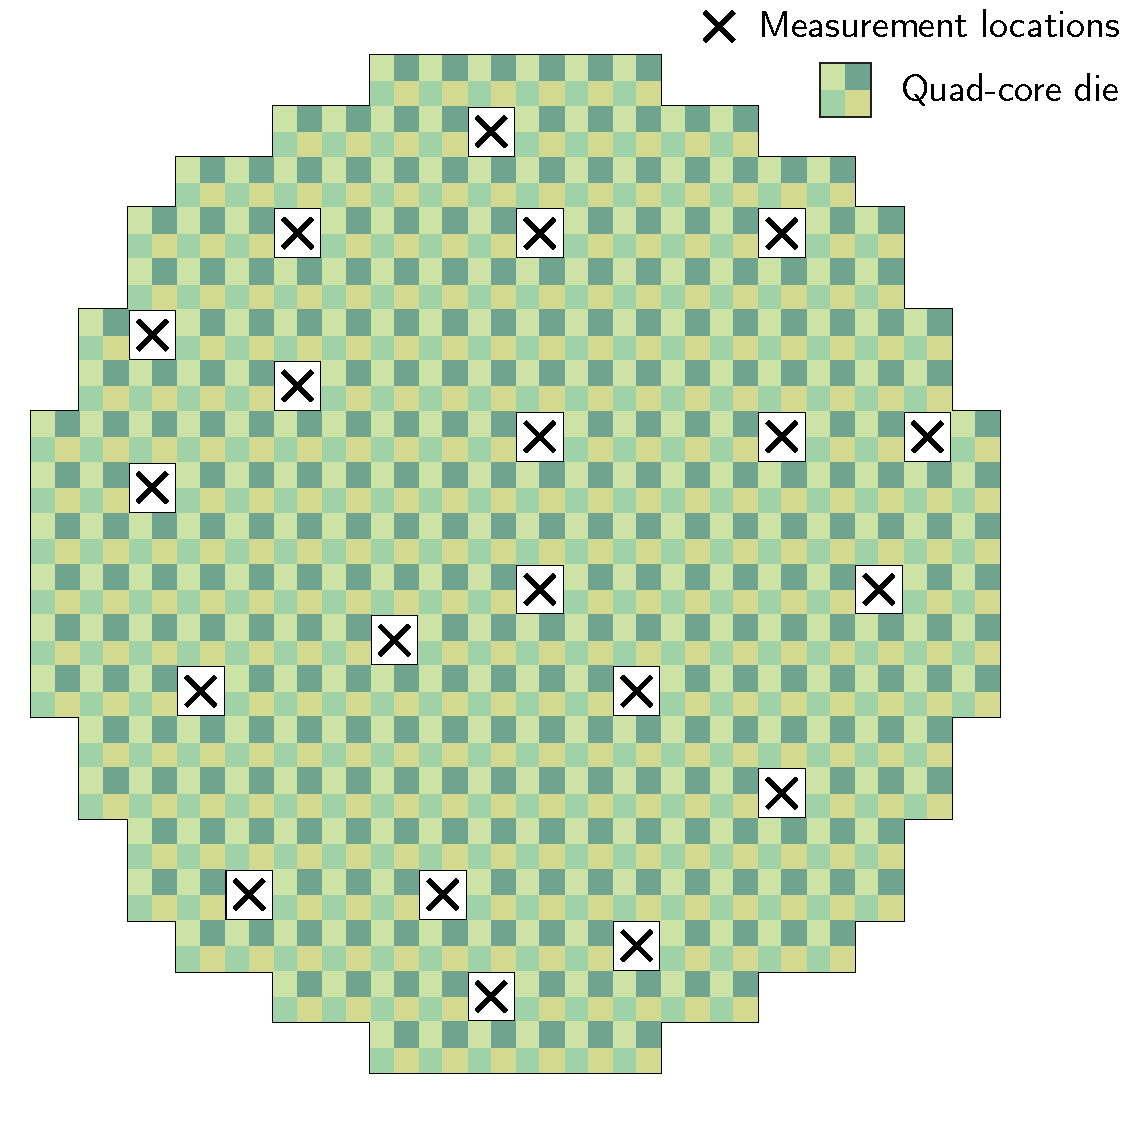
\includegraphics[width=0.7\linewidth]{include/assets/wafer-pick.pdf}
  \caption{A wafer with 316 quad-core dies.}
  \flabel{wafer-pick}
  \vspace{-1.5em}
\end{figure}

\begin{figure}
  \centering
  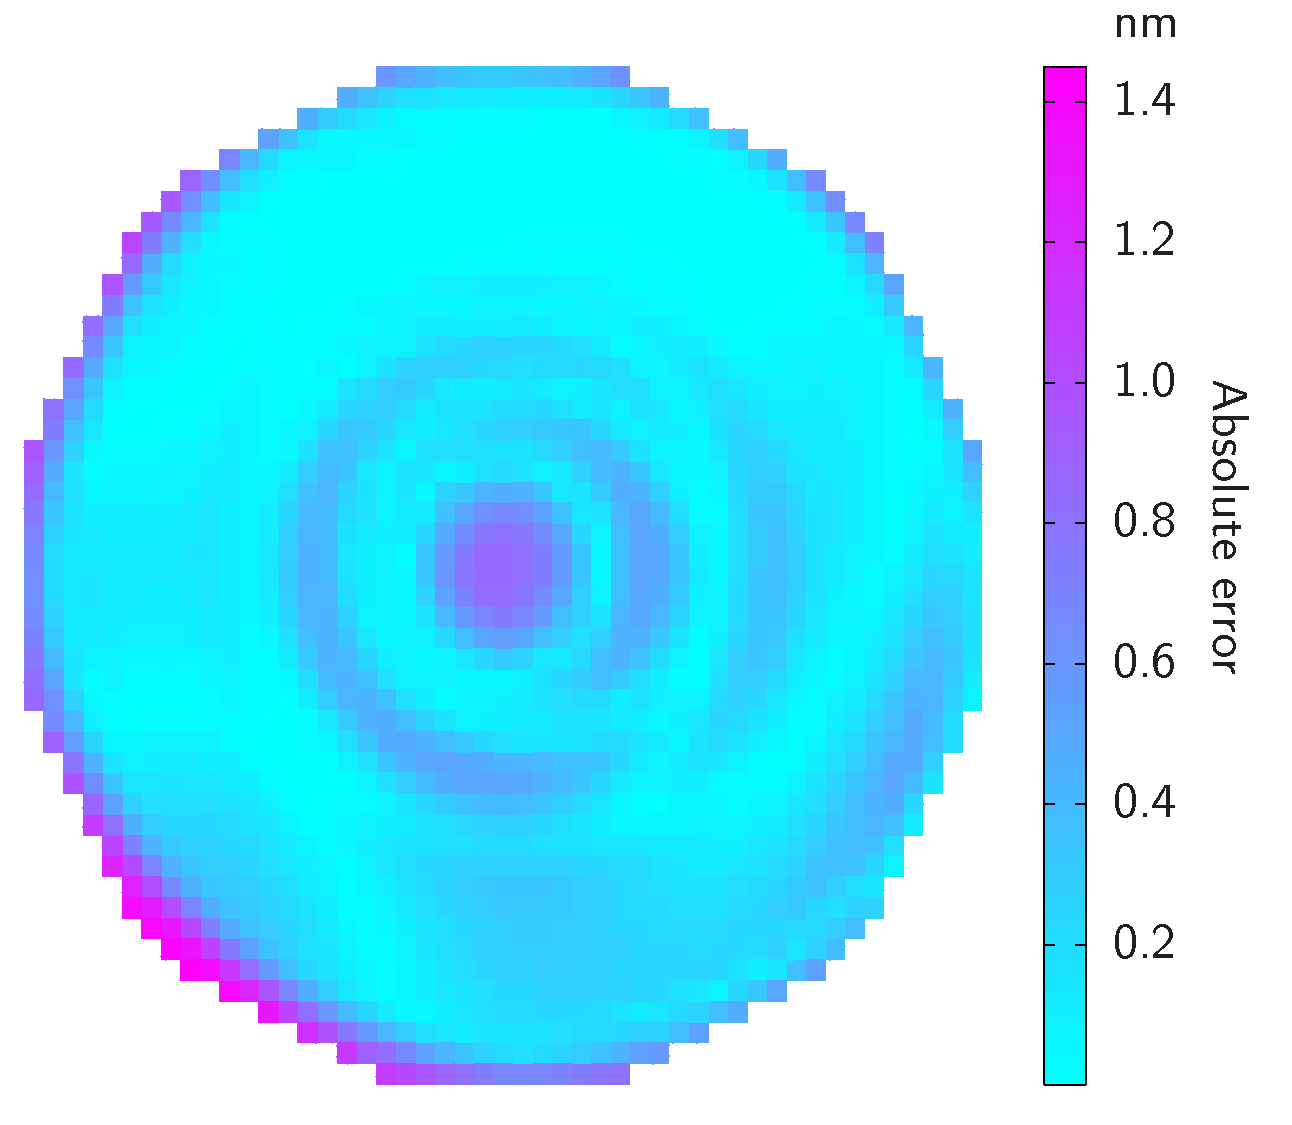
\includegraphics[width=0.6\linewidth]{include/figures/wafer-qoi-error.pdf}
  \caption{Absolute error across the wafer.}
  \flabel{wafer-qoi-error}
\end{figure}

Now, we shall describe the default configuration of our experimental setup, which, in the following subsections, will be adjusted according to the purpose of a particular experiment. We consider a 45-nanometer technological process. The wafer is assumed to be inscribed in a square with $20 \times 20$ even cells. The total number of dies $\nchips$ is 316, and the number of processing elements $\nprocs$ on each of the dies is four. The number of spacial measurements $\ndata$ is 20. These locations (dies) are chosen as follows: the first one is place in the middle of the wafer, and the rest are selected sequentially such that the total distance from the already picked dies and the new one to the left dies is minimized. In this way, we pursue uniformity of the wafer coverage. An example is depicted in \fref{wafer-pick}. The floorplans of the multiprocessor platforms are constructed in such a way that the processing elements form regular grids, as it is the case with, \eg, Alpha 21264 studied in \cite{juan2011}. The capacitance and conductance matrices in \eref{heat-de} are obtain using HotSpot v5.02 \cite{hotspot}. The dynamic power profiles involved in the experiments are based on simulations of randomly generated task graphs using TGFF v3.5 \cite{dick1998}.\footnote{The floorplans of the platforms, thermal configuration of HotSpot, task graphs of the applications, etc. are available online at \cite{sources}.} The sampling interval of these profiles is $1~\text{ms}$. The number of temporal measurements $\nsteps$ is 20. These time moments are chosen to be evenly spaced and to cover the whole time spans of the corresponding dynamic power profiles  $\profilePdyn$ (the total number of steps $\npsteps$ is typically much larger).

Let us turn to the statistical model in \sref{statistical-model}. In the covariance function given by \eref{covariance-function}, the weight parameter $\eta$ is 0.7 prioritizing the squared exponential kernel, and both length-scale parameters, $\ell_\SE$ and $\ell_\OU$, are set to half the radius of the wafer. The threshold parameter in the model order reduction procedure described in \sref{kl-expansion} is set to $0.99$ preserving $99\%$ of the variance of the data; the number of the resulting \rvs, \ie, the dimensionality of $\vz$ in \eref{kl-approximation}, $\nvars$, was found to be around 27. In the prior for the mean of $\u$ (see \eref{mu-u-prior}), we let $\mu_0$ be $45~\text{nm}$ and $\sigma_0$ be $1\%$ of $\mu_0$. The later represents our rather high certainty about the expected value of $\u$ as it is a part of the specification of the technological process. In the prior for the variance of $\u$ (see \eref{sigma2-u-prior}), we let $\tau_\u$ be $5\%$ of the mean value \cite{juan2011, juan2012}, and $\nu_\u$ is set to ten. The later has an intuitive interpretation in the Bayesian context: $\nu_\u$ can be thought of as being the number of imaginary observations (prior to actual observations) that the decision about $\tau_\u$ is based on. In the prior for the variance of noise (see \eref{sigma2-noise-prior}), we let $\tau_\noise$ be $1~\text{K}$ (Kelvin), and $\nu_\noise$ be ten observations (the same meaning as for $\nu_\u$). To summarize the reasoning behind the priors, the hyperparameters $\mu_0$, $\tau_\u$, and $\tau_\u$ represent the presumable values of $\mu_u$, $\sigma_\u$, and $\sigma_\noise$, respectively, and the hyperparameters $\sigma_0$, $\nu_\u$, and $\nu_\noise$ reflect the degree of our beliefs according to our prior knowledge. In the absence of such knowledge, non-informative priors can be chosen; refer to \cite{gelman2004} for further details. The tuning constant $\alpha$ in \eref{proposal} is set to 0.5. The optimization procedure (recall \sref{proposal-distribution}) is limited by $10^4$ objective function evaluations (the log-posterior in \eref{log-posterior}). The number of samples that we draw from the posterior is $10^4$; the first half of these samples is discarded leaving $5 \cdot 10^3$ effective samples $\nsamples$. Unless otherwise stated, the number of processes performing the Metropolis sampling in parallel is four.\footnote{All the experiments have been conducted on a GNU/Linux machine with Intel Core i7 2.66~GHz and 8~GB of RAM.}

\subsection{In-depth Analysis}
\begin{figure}
  \centering
  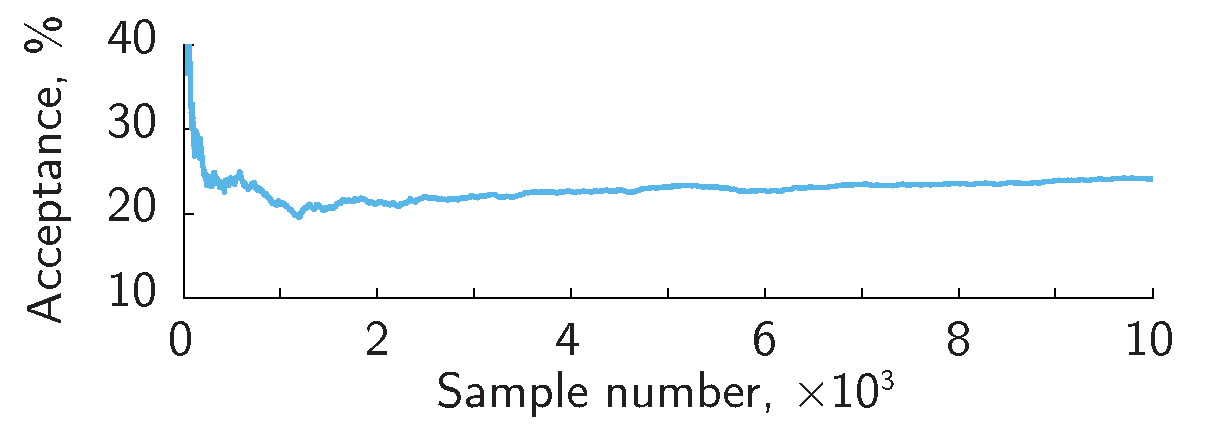
\includegraphics[width=0.7\linewidth]{include/figures/acceptance.pdf}
  \caption{Evolution of the acceptance rate.}
  \flabel{acceptance}
  \vspace{-0.5em}
\end{figure}

\begin{figure}
  \centering
  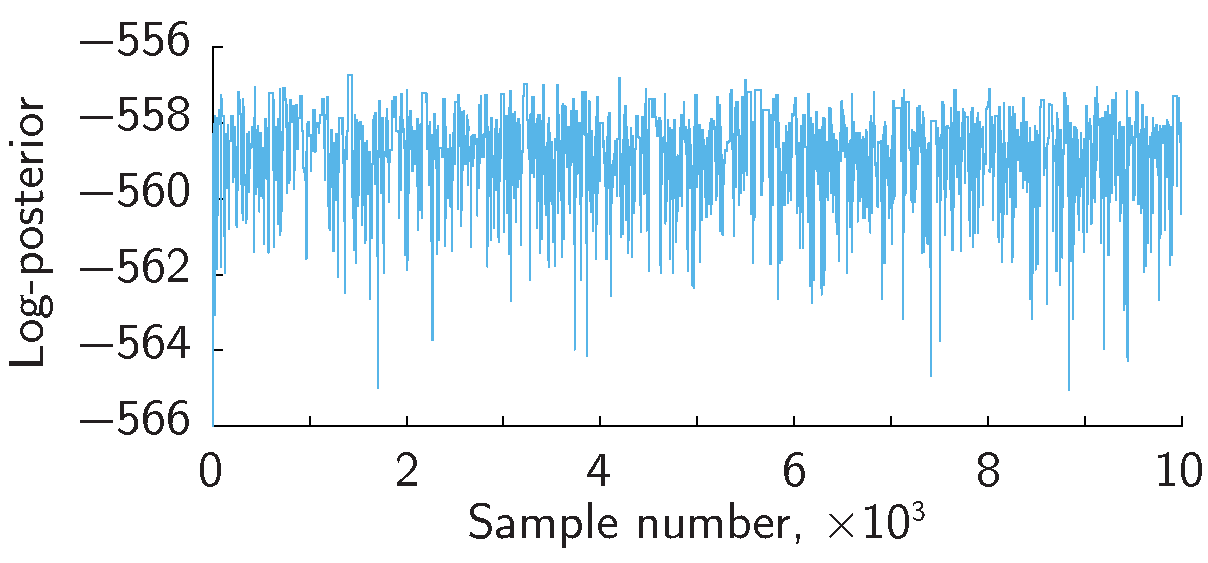
\includegraphics[width=0.7\linewidth]{include/assets/log-posterior.pdf}
  \caption{Evolution of the log-posterior.}
  \flabel{log-posterior}
  \vspace{-1.5em}
\end{figure}

\begin{figure}
  \centering
  \vspace{-1.5em}
  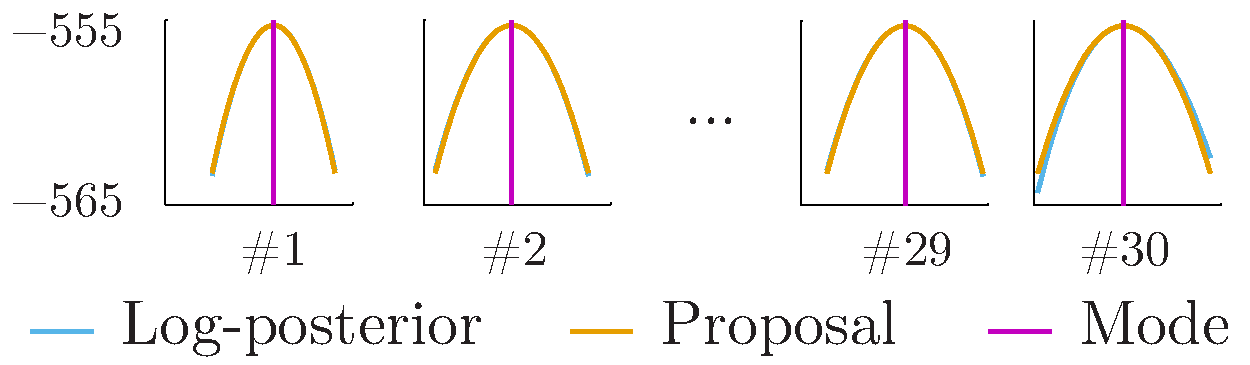
\includegraphics[width=0.8\linewidth]{include/figures/proposal.pdf}
  \caption{Inspection of the proposal.}
  \flabel{proposal}
\end{figure}

Let us first perform a detailed analysis of the results obtained for one particular example with the default configuration described earlier. The true and inferred distributions of the QoI are shown in \fref{wafer-qoi}. In this case, the normalized root-mean-square error (NRMSE) is below $2.8\%$, and the distribution across the wafer of the absolute error can be observed in \fref{wafer-qoi-error}. It can be seen that the framework produces a close match to the true value of the QoI. The graph in \fref{acceptance} displays the acceptance rate of the Metropolis algorithm, from which we conclude that algorithm, accepting $20$--$30\%$ of samples on average, agrees with the recommendations from the literature \cite{gelman2004}. We can also conclude that the constructed Markov chain vividly explores the probability space by looking at the log-posterior (up to a constant summand) in \fref{log-posterior}. One more test, common in statistics, to assess the quality of the proposal distribution is given in \fref{proposal}. Here, the proposal in \eref{proposal} is plotted along with the log-posterior in \eref{log-posterior} around the posterior mode $\hat{\vparam}$. Since, in this example, the dimension of $\vparam$ is 30, the number of such plots is also 30. The curves are nearly indistinguishable implying a high quality of the proposal. The above premises lead to the conclusion that the optimization and sampling procedures are fine-tuned.

\subsection{Number of Processing Elements}
In this subsection, we consider five platforms with the number of processing elements $\nprocs$ equal to 2, 4, 8, 16, and 32 cores, respectively. The results are summarized in \tref{processing-elements}.
\begin{table}[h]
  \centering
  \caption{Results for the number of processors $\nprocs$.}
  \begin{tabular*}{0.90\linewidth}{lrrrrr}
    \toprule
    Processing elements & 2 & 4 & 8 & 16 & 32 \\
    \midrule
    Time in sequence, m & 0 & 0 & 0 & 0 & 0 \\
    Time in parallel, m & 1.87 & 2.71 & 5.36 & 10.09 & 26.32 \\
    NRMSE, \%           & 4.50 & 3.62 & 3.92 &  2.69 &  1.82 \\
    \bottomrule
  \end{tabular*}
  \tlabel{processing-elements}
  \vspace{-1em}
\end{table}


\subsection{Number of Space Measurements}
In this subsection, we change the number of dies $\ndata$ for which the measurement data are available in the input data set $\Data$ (correspondingly, $\nchips - \ndata$ dies on the wafer are left unobserved). The considered scenarios are 1, 10, 20, 40, 80, and 160 dies.

\subsection{Number of Time Measurements}
In this subsection, we sweep the number of moments of time $\nsteps$ for which the measurement data are available in the input data set $\Data$ (correspondingly, $\npsteps - \nsteps$ steps are discarded after $\model$ is evaluated for the input power profile $\profilePdyn$). The considered scenarios are 1, 10, 20, 40, 80, and 160 moments of time.

\subsection{Measurement Noise}
In this subsection, we vary the level of the noise in the input data set $\Data$ within the set $\{ 0, 0.5, 1, 2 \}$ (in Kelvins) while keeping the corresponding prior distribution in \eref{sigma2-noise-prior} unchanged.

\subsection{Numerical vs. Analytical Solution}
In this subsection, we demonstrate the speedup due to the analytical solution of the forward model comparing with a numerical solution (see \sref{analytical-solution}).

\subsection{Na\"{i}ve vs. Optimized Proposal Distribution}
In this subsection, we show the importance of the optimization procedure preceding the sampling part (see \sref{proposal-distribution}).

\subsection{Sequential vs. Parallel Sampling}
In this subsection, we illustrate the difference between the two sampling strategies: sequential and parallel (see \sref{sampling-strategy}). Since the limit on the number of objective function evaluations of the optimization procedure and the number of sample draws (including the burn-in prior) is the same, \ie, equal to $10^4$, the two would take the same time to finish if the optimization reached the limit. In our experiments, however, this limit was never observed to be reached. Therefore, using the default setup without parallelization, the optimization always takes less time than sampling. The situation changes when parallel computing (with four workers, in our case) is plugged in: the sampling part decreases by approximately 2–3 times, which indicates good parallelization properties of the chosen sampling strategy.


  \section{Conclusion} \slabel{conclusion}
  In this paper, we proposed a novel framework for the analysis of process variation across semiconductor wafers, which is based on cost-efficient indirect measurements analyzed via Bayesian inference.
The technique was exposed to an extensive study of various aspects concerning its practical implementation.
The obtained findings support the computational efficiency and accuracy of our approach.

As a closing remark, we would like to note that, although the framework was demonstrated on the effective channel length, it can be readily utilized to analyze any other \qois\ affected by process variation and, moreover, to study their combinations.
In addition, the user is free to replace the data model described in \sref{data-model}, which consists of the power and temperature components, with another model, serving the same purpose, if this change is considered to be more beneficial in a certain particular context.


  \begingroup
  \setlength\bibitemsep{2pt}
  \printbibliography
  \endgroup
\end{document}

% vim: ft=tex
